% ATIVIDADES REALIZADAS------------------------------------------------------------------

\chapter{Atividades realizadas}
\label{chap:atividadesRealizadas}

Nesse capítulo será explanada minha participação no processo de desenvolvimento do projeto o qual tive a oportunidade de participar desde a concepção, homologação, correção de problemas, criação de uma nova versão com expressiva mudança no modelo de dados até a implementação da aplicação em produção.

\section{\imprimirtitulo}
\label{sec:atividadesRealizadasVeiculos}

O projeto \imprimirtitulo \space foi concebido com o objetivo de controlar as solicitações de veículos e as viagens realizadas, promovendo uma melhor gestão da frota de veículos do TRE-PB bem como possibilitando a realização de auditorias com base nos dados contidos no sistema.
O sistema é hoje um ativo de TI que foi desenvolvido pela SEDES e está descrito no catálogo técnico de sistemas da COSIS conforme \autoref{fig:figura-ativoTI}. 

\begin{figure}[!htb]
    \centering
    \caption{Catálogo técnico de sistemas - Veículos}
    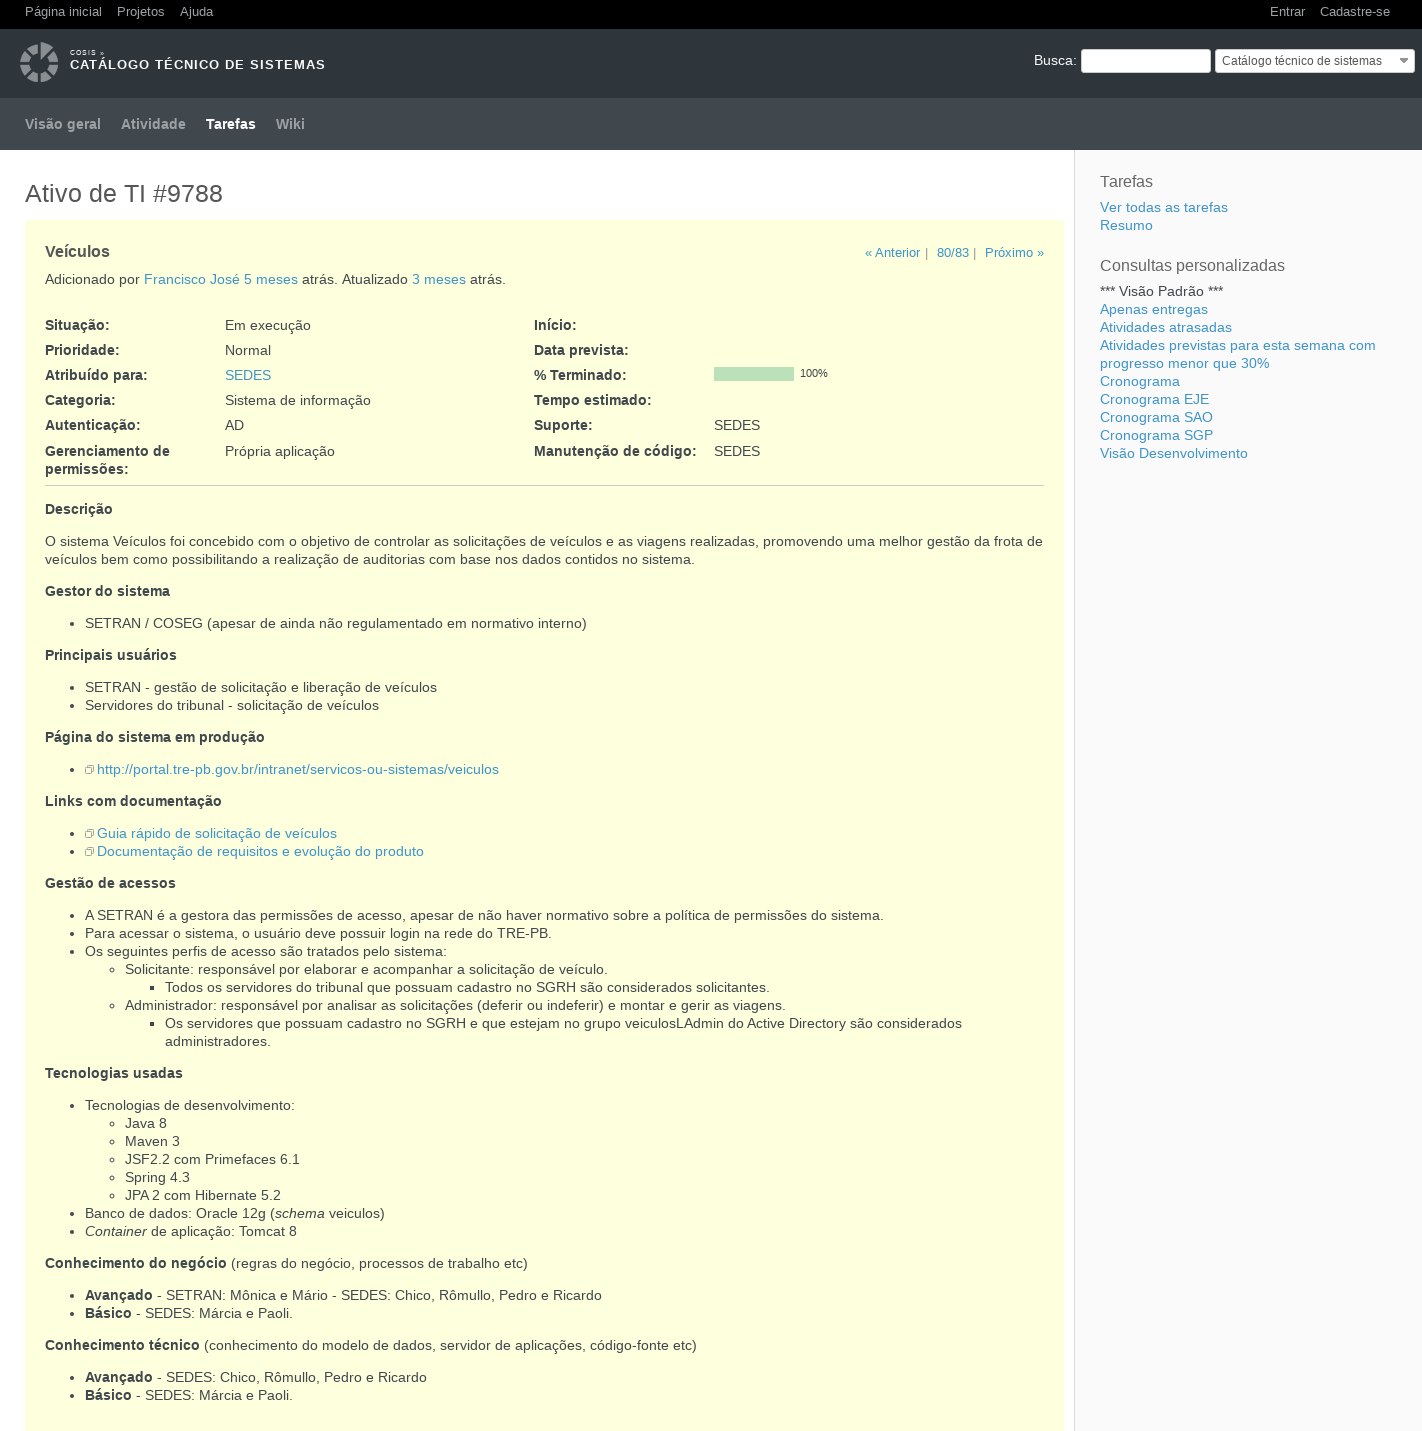
\includegraphics[width=0.75\textwidth]{./dados/figuras/veiculos-ativoTI}
    \fonte{COSIS}
    \label{fig:figura-ativoTI}
\end{figure}

O sistema permite a qualquer membro e servidor lotado no TRE-PB, através do seu login de usuário, solicitar um veículo descrevendo a data, local/trecho, hora de partida, hora de retorno, a atividade que deverá ser realizada e quais passageiros irão para o mesmo destino, como pode ser visto na \autoref{fig:figura-solicitacao}.

\begin{figure}[!htb]
    \centering
    \caption{Veículos - Tela de solicitação}
    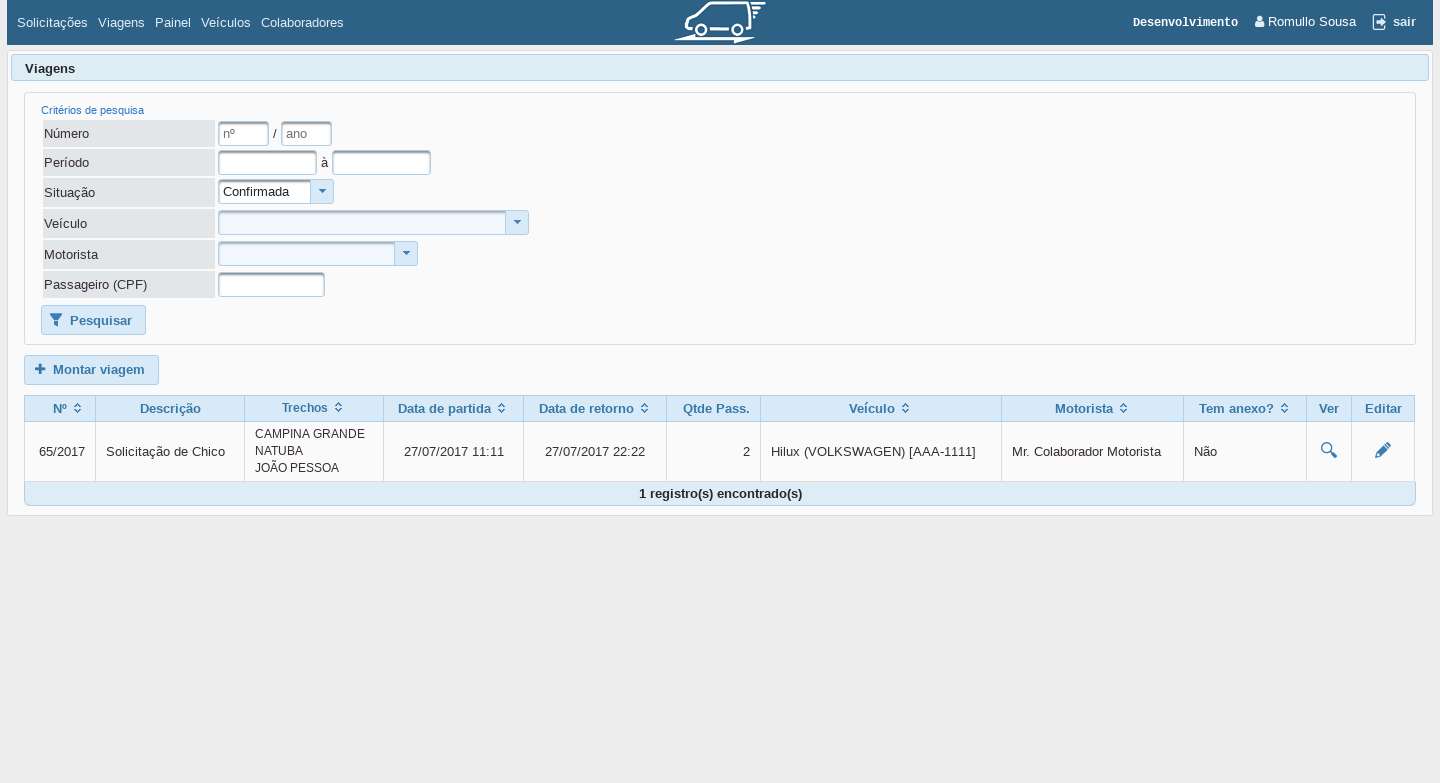
\includegraphics[width=0.75\textwidth]{./dados/figuras/veiculos-tela1.png}
    \fonte{SEDES}
    \label{fig:figura-solicitacao}
\end{figure}

O gestor lotado na SETRAN, possui um perfil de administrador e em sua tela recebe as solicitações de todos os servidores e membros. Com a visão de todas as solicitações o gestor tem a possibilidade de analisar passageiros que irão para os mesmos destinos, ou até mesmo na rota, com horários similares e montar as viagens adequando a disponibilidade de motoristas e veículos. Através de um quadro, exibido na figura \autoref{fig:figura-motoristas}, o gestor consegue visualizar a ocupação dos veículos e motoristas pelo horário e dia da semana. Com a viagem montada e deferida pelo gestor, o solicitante recebe uma confirmação em seu e-mail informando os detalhes da viagem. Os motoristas recebem uma guia contendo a autorização e detalhes da viagem como a rota e os passageiros. Nessa guia o motorista deve anotar a quilometragem do veículo e exibir para o vigia que deve conferir os valores e permitir a saída do veículo. No retorno o motorista novamente anota na guia a quilometragem de chegada que é conferida pelo vigia.

A modelagem inicial do sistema, na versão 1.0.0, não possuia uma separação dos modelos entre solicitação e viagem. Isso acabou ocasionando um gargalo no desenvolvimento, pois surgiram feedbacks ao longo das etapas, como pode ser visto na ata de reunião na \autoref{fig:figura-ata1}, em que há casos de uma solicitação necessitar de mais de uma viagem para ser concluída e uma viagem poder atender mais de uma solicitação. A aplicação precisou ser refatorada e um novo prazo foi apresentado.

\begin{figure}[!htb]
    \centering
    \caption{Veículos - Tela de solicitação}
    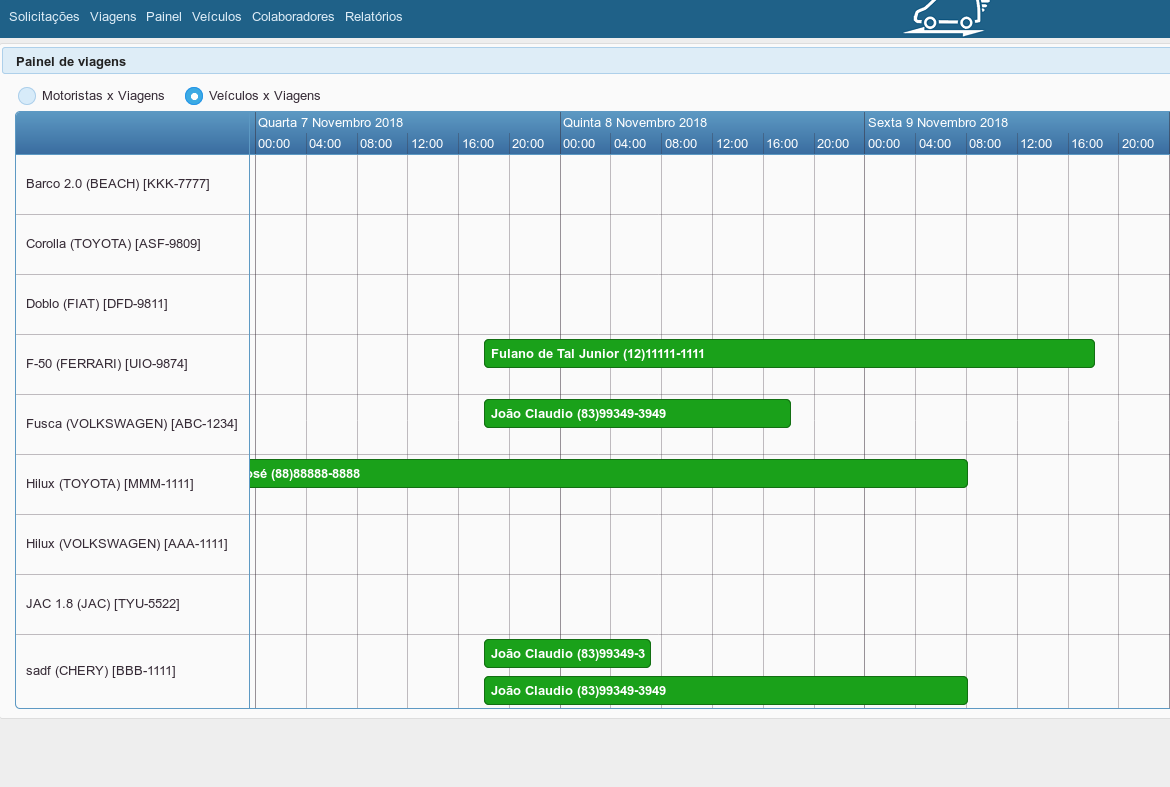
\includegraphics[width=0.75\textwidth]{./dados/figuras/veiculos-tela2.png}
    \fonte{SEDES}
    \label{fig:figura-motoristas}
\end{figure}

\begin{figure}[!htb]
    \centering
    \caption{Ata de reunião - feedback}
    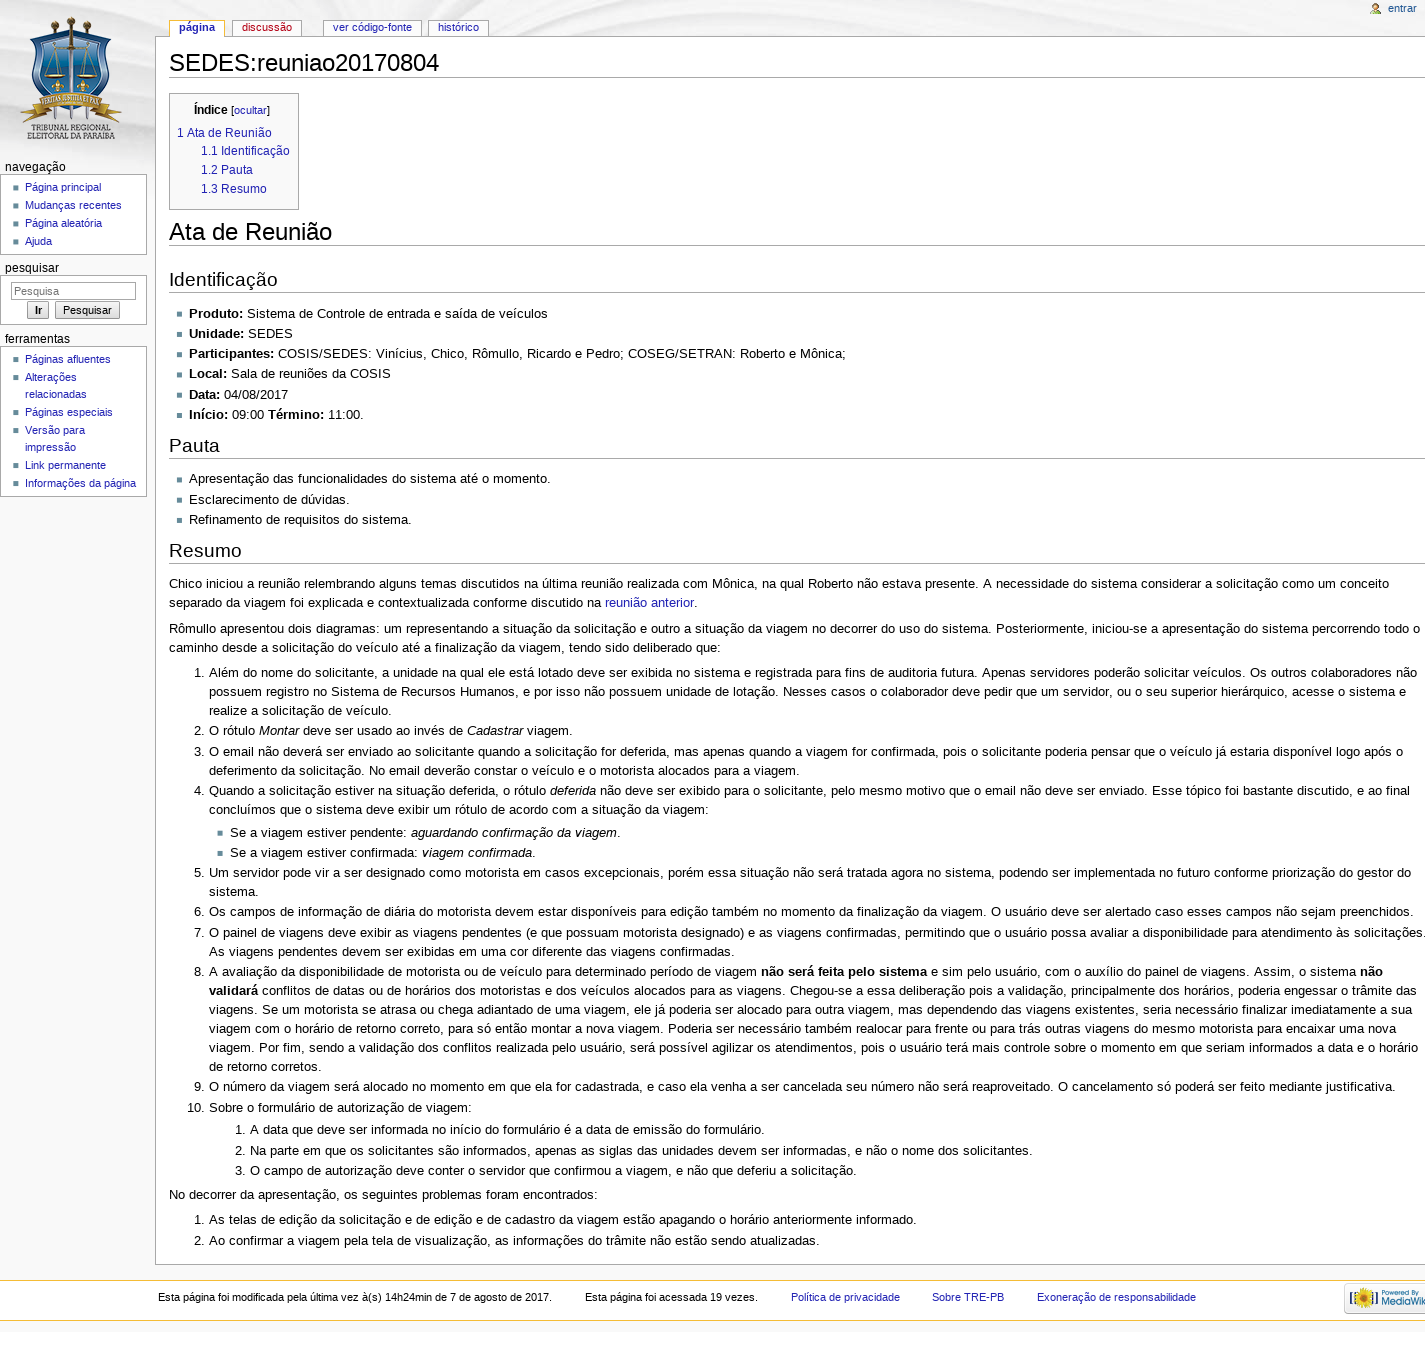
\includegraphics[width=1\textwidth]{./dados/figuras/veiculos-ata1.png}
    \fonte{SEDES}
    \label{fig:figura-ata1}
\end{figure}

O desenvolvimento do sistema passou por todas as etapas de um projeto de software conforme descrição no modelo de desenvolvimento de software no Anexo \ref{chap:anexoA}. Esse modelo foi construído a partir de definições estabelecidas em portarias, conforme exemplo, no Anexo \ref{chap:anexoB} da última publicada pela Diretoria Geral do TRE-PB no que se diz respeito aos padrões de governança em Tecnologia da Informação.
O processo de desenvolvimento e manutenção de software se inicia com a autorização de análise do problema, visando à elaboração de proposta de solução  \cite[p.~2]{Portaria37:2017}.
 

\section{A análise do problema}
\label{sec:atividadesRealizadasInicio}

Uma reunião inicial é realizada entre todos os interessados. A COSIS reúne o gestor do sistema, o time de desenvolvimento e o cliente. 

Para o time já se inicia o processo de imersão, onde após ouvir as necessidades descritas pelo cliente começa a imaginar e descrever os possíveis requisitos necessários para a solução. 
Toda reunião realizada entre a equipe e o cliente é descrita cronologicamente e fica publicada na categoria de Atas/Reuniões da SEDES na sitio Wiki do TRE-PB, com a data, hora de início e fim e o nome de todos os participantes, conforme \autoref{fig:figura-ataReuniao1}. Dessa forma todos tem acesso ao que realmente foi solicitado.

\begin{figure}[!htb]
    \centering
    \caption{Ata de Reunião - 21/03/2017}
    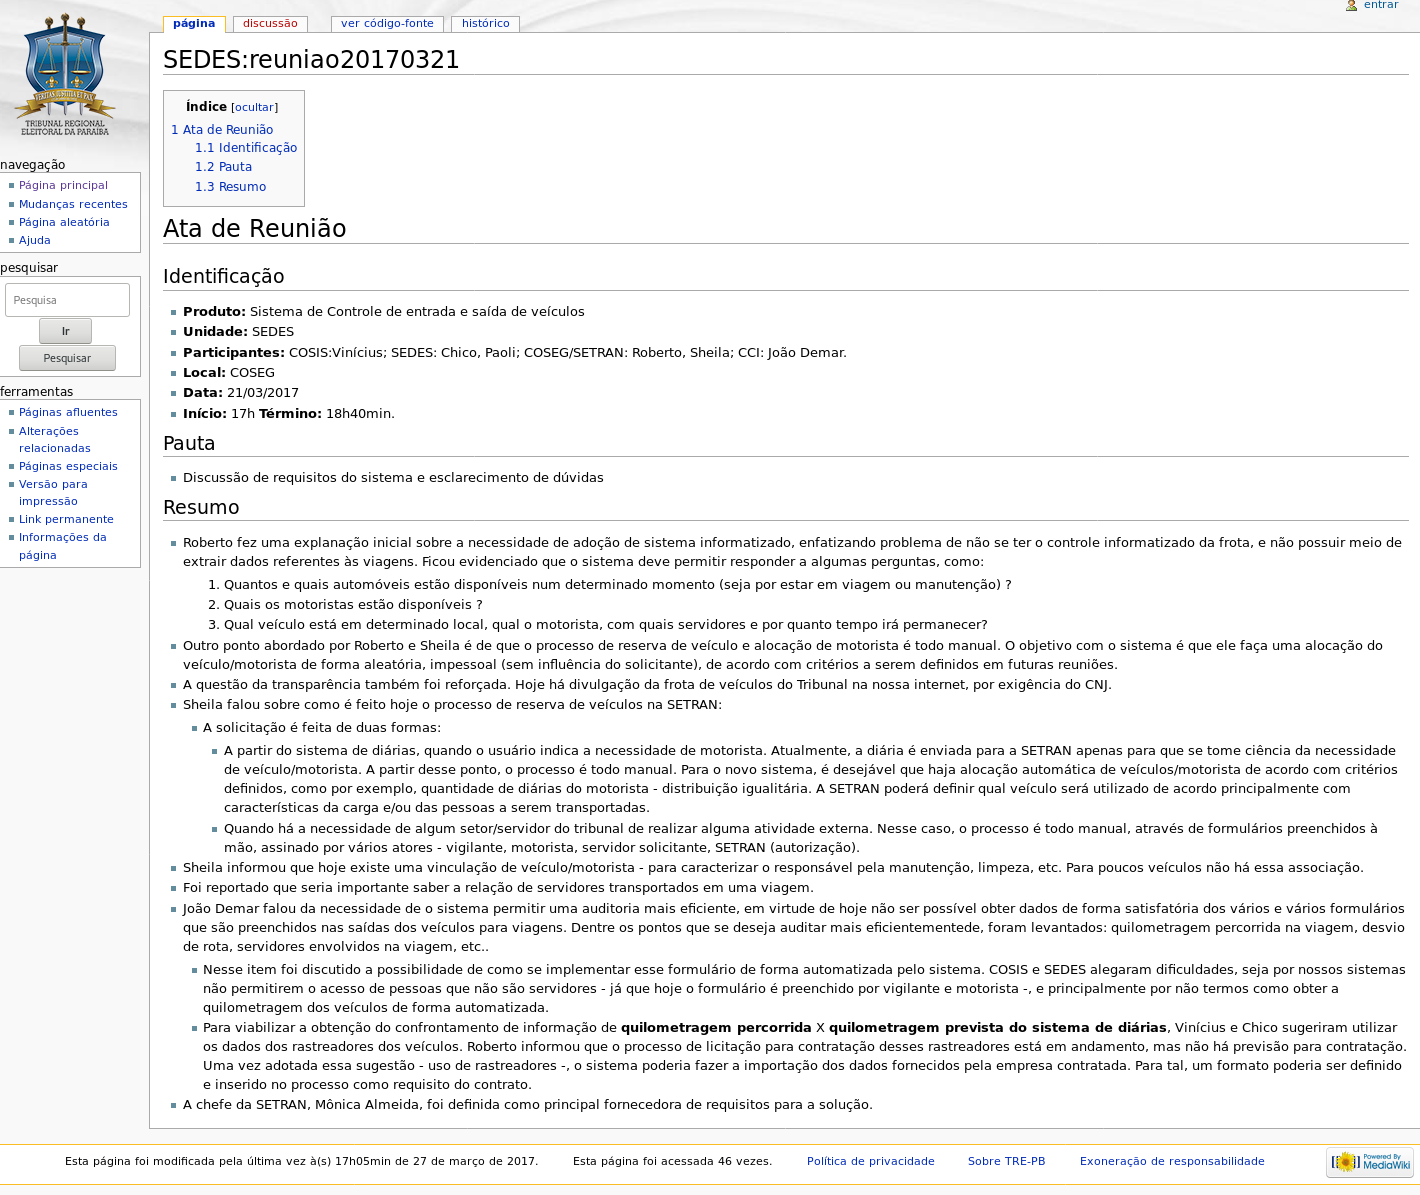
\includegraphics[width=0.9\textwidth]{dados/figuras/veiculos-reuniao20170321}
    \fonte{SEDES}
    \label{fig:figura-ataReuniao1}
\end{figure}

Posteriormente o time volta a se reunir e descrever as histórias de usuário na forma de requisitos a serem implementados. Com os requisitos descritos e cadastrados no sistema de gestão de projetos, o Redmine, na forma de tarefas e atividades, é possível mensurar o tamanho de cada atividade e assim estimar o tempo necessário para conclusão do projeto.  

\section{Planejamento}
\label{sec:atividadesRealizadasPlanejamento}

Todos os membros do time se reúnem para medir o tamanho de cada atividade. Uma a uma, as atividades são analisadas e discutidas por cada membro do time onde cada um expõe sua opinião e justifica o tamanho da atividade mensurada através da técnica do Planning Poker. Após um consenso entre todos, fica definido o tamanho da atividade. Assim o gerente, com esses dados em mãos, formaliza o projeto como uma demanda de serviço, contendo o prazo e o time necessário para concluir as releases.

\begin{citacao}
Após a autorização, o gestor do sistema promoverá a reunião de
partida entre o time de desenvolvimento e as partes interessadas, momento em que será
esclarecido o problema de negócio, definidos papéis, explicado o processo de
desenvolvimento e distribuídas responsabilidades.\cite[p.~2]{Portaria37:2017}
\end{citacao}

As releases definidas são apresentadas como as versões que serão entregues e são separadas conforme ordem de prioridade das atividades e requisitos como mostra a \autoref{fig:figura-planejamento}.


\begin{figure}[!htb]
    \centering
    \caption{Planejamento das versões}
    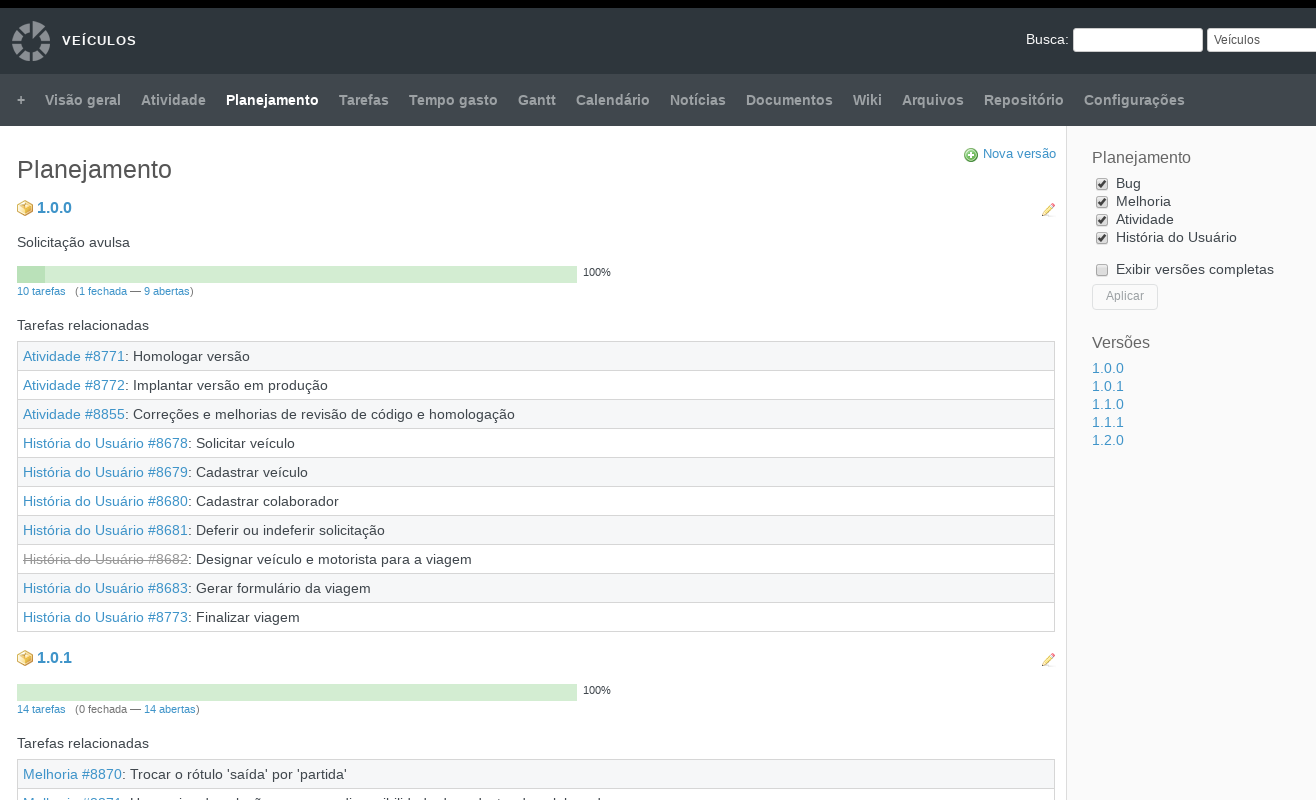
\includegraphics[width=0.75\textwidth]{dados/figuras/veiculos-planejamento.png}
    \fonte{SEDES}
    \label{fig:figura-planejamento}
\end{figure}

\section{Desenvolvimento}
\label{sec:atividadesRealizadasDesenvolvimento}

No início da fase de desenvolvimento são gerados os primeiros artefatos em código que serão comuns para todos os membros do time. O TRE-PB utiliza para controle de versões de seus códigos o sistema de versionamento denominado Subversion (SVN). Um novo repositório é criado para o projeto e um novo projeto com um arcabouço contendo as bibliotecas padrões e um template para as páginas já utilizadas pela SEDES é criado e disponibilizado no repositório para todos os desenvolvedores. A SISBAN. que através de um chamado, gera um novo schema no banco de dados Oracle 12g e fornece acesso a todos os desenvolvedores.

Todo esse processo é inicialmente implementado pelo supervisor técnico que geralmente é o desenvolvedor responsável pelo projeto e com mais habilidades e experiência do time.

Nesse momento todas as histórias já estão descritas com uma riqueza maior de detalhes, então são criados tickets e colados em um taskboard na forma de um quadro Kanban visível para todos. Esse quadro contém todas as atividades necessárias que atendem ao escopo do projeto para a release em questão. 

Diariamente são realizadas pequenas reuniões denominadas "daily" entre o gestor do projeto e membros do time com o intuito de detalhar o andamento das atividades, conduzir novas atividades para o time bem como relatar as dificuldades encontradas.

Na \autoref{fig:figura-atividade8940} a seguir é possível ver uma tarefa especifica que foi atribuída a mim. A tarefa cadastrada no Redmine possui uma ligação com o repositório SVN, assim é possível ver e analisar trechos de códigos que foram implementados em cada "commit"\footnote{No contexto de ciência da computação e gerenciamento de dados, commit refere-se à ideia de fazer permanentes um conjunto de mudanças experimentais. Uma utilização popular está no fim de uma transação. Um commit é o ato de enviar. https://pt.wikipedia.org/wiki/Commit}.

\begin{figure}[!htb]
    \centering
    \caption{Atividade 8940}
    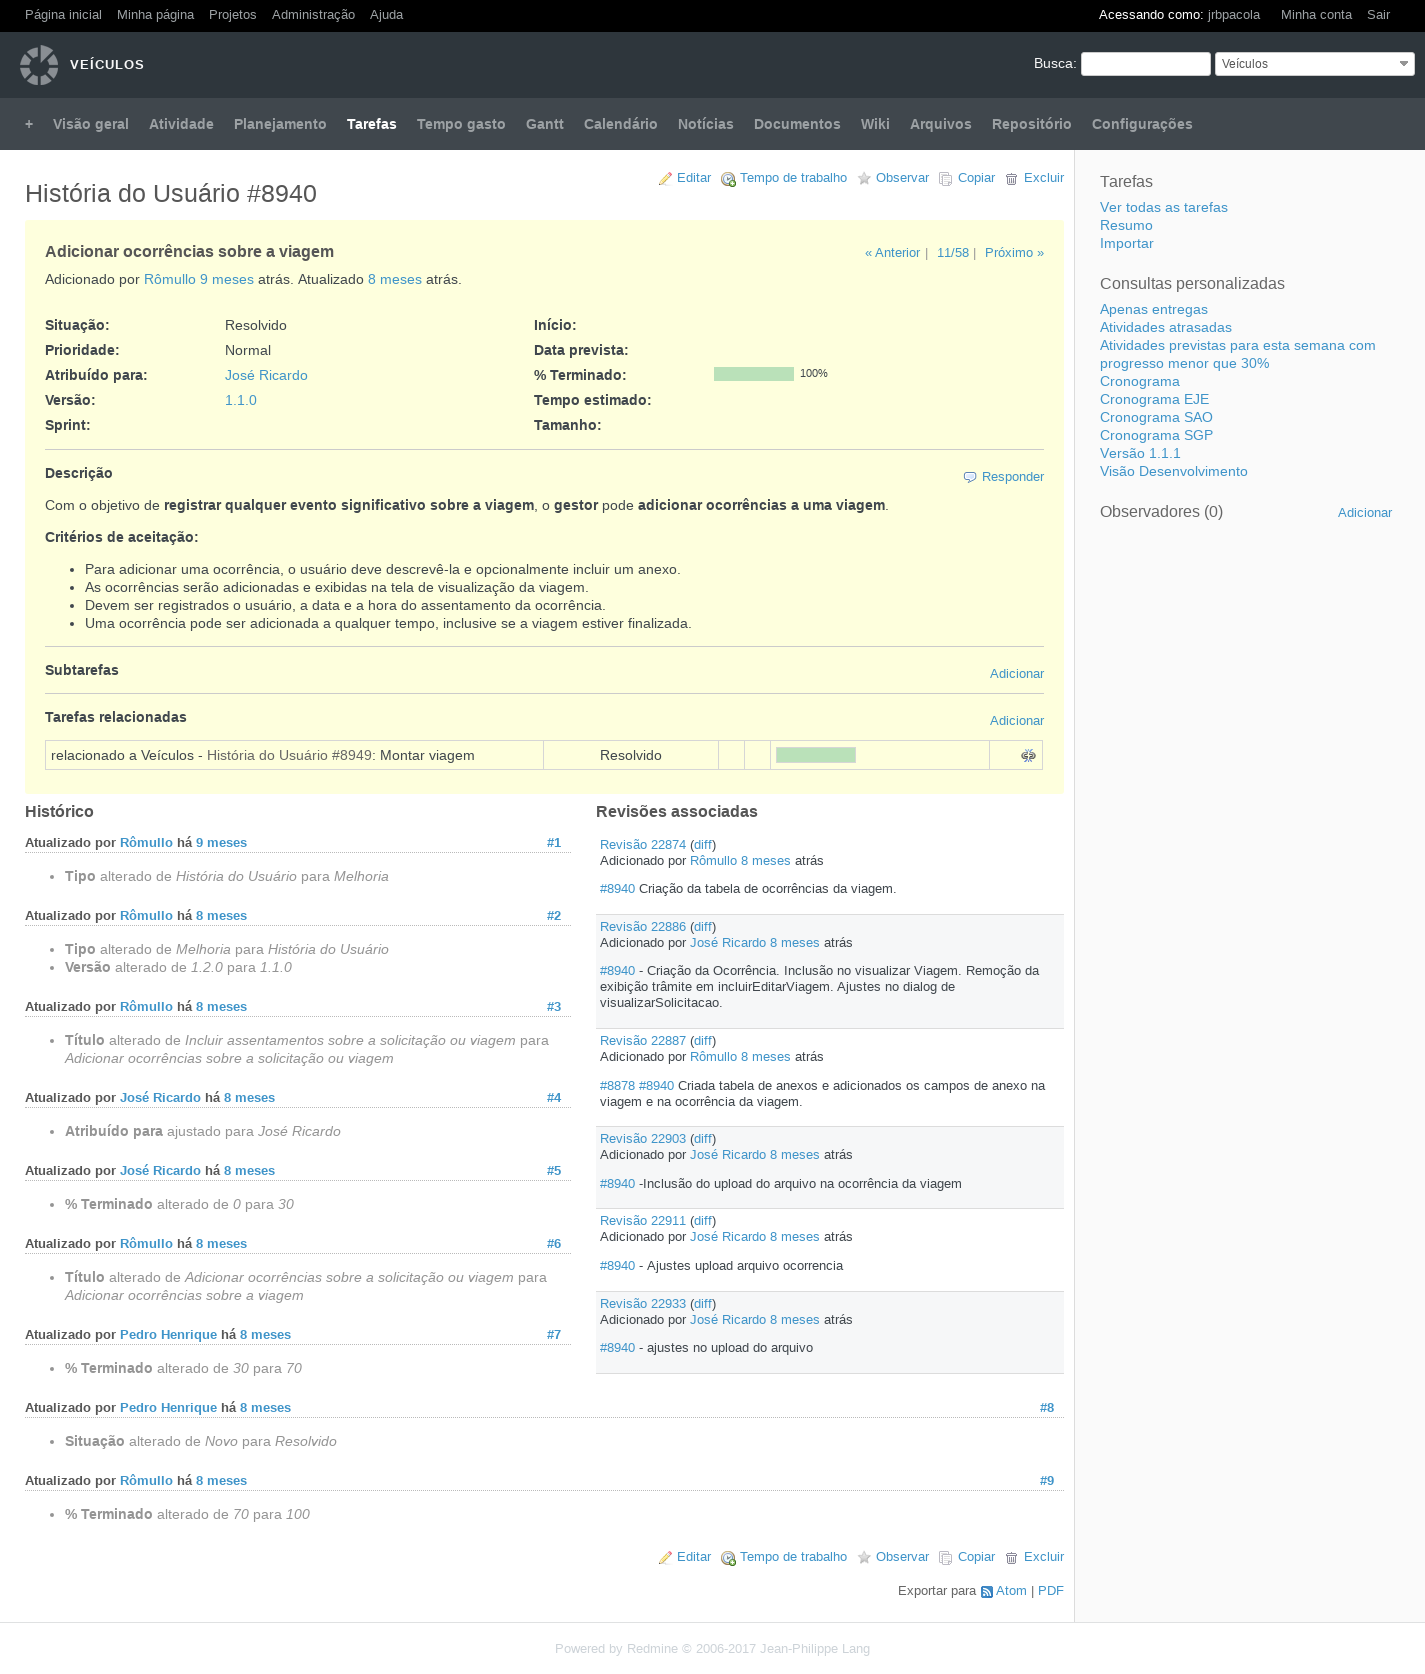
\includegraphics[width=0.75\textwidth]{dados/figuras/veiculos-atividade1.png}
    \fonte{SEDES}
    \label{fig:figura-atividade8940}
\end{figure}


\subsection{Criando as tabelas no banco}
\label{sbs:desenvolvimentoTabelas}

Com o domínio do problema já definido são então criadas as tabelas do banco de dados com seus atributos, relacionamentos e restrições.
Scripts em SQL são gerados, conforme exemplo da \autoref{fig:figura-scriptSQL}, para cada tabela, levando em consideração as particularidades da sintaxe SQL para o banco de dados Oracle. 

\begin{figure}[!htb]
    \centering
    \caption{Script SQL}
    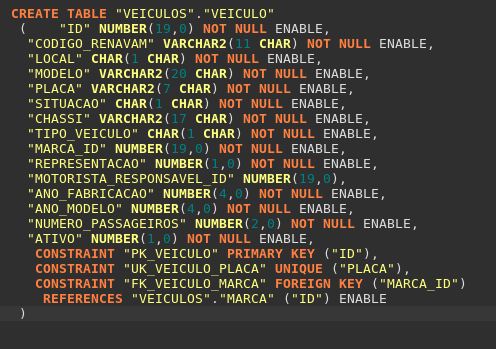
\includegraphics[width=0.75\textwidth]{dados/figuras/scriptSQL.png}
    \fonte{SEDES}
    \label{fig:figura-scriptSQL}
\end{figure}

\subsection{Mapeando o modelo com o banco}
\label{sbs:desenvolvimentoMapeamento}

Com as tabelas já criadas e relacionadas, começa-se a codificação propriamente dita na linguagem Java. As classes do modelo são codificadas com seus respectivos atributos e métodos e mapeadas através da interface JPA. Na \autoref{fig:figura-entidade} é possível ver a entidade que define um veículo na aplicação já com as anotações que a mapeiam com o banco de dados.

\begin{figure}[!htb]
    \centering
    \caption{Entidade Java - Veículo}
    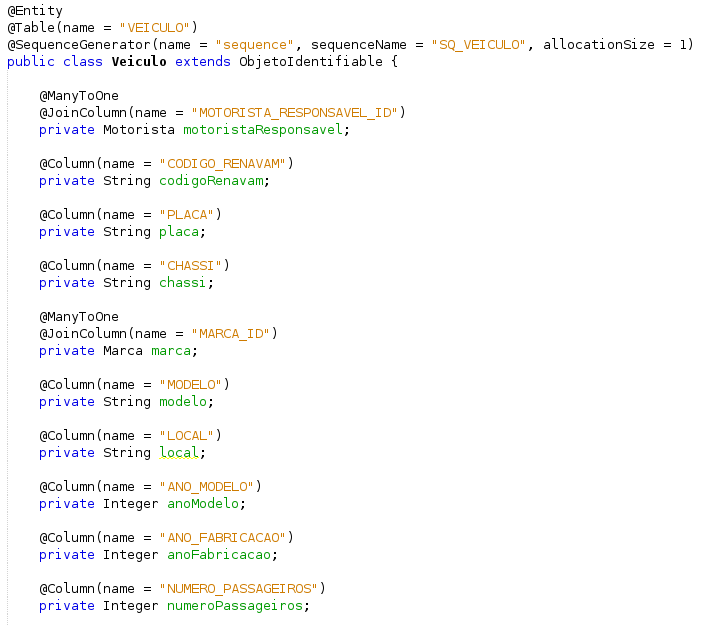
\includegraphics[width=0.75\textwidth]{dados/figuras/entidade.png}
    \fonte{SEDES}
    \label{fig:figura-entidade}
\end{figure}

\subsection{MVC}

As aplicações em Web desenvolvidas no TRE-PB que utilizam o JEE obedecem o padrão de projeto denominado MVC. O código tem uma divisão lógica. 
Na camada de modelo(Model) temos as entidades que definem o domínio da aplicação como pode ser visto na \autoref{sbs:desenvolvimentoMapeamento}. 
Na camada de visão(View) da aplicação temos as páginas JSF que irão conter os componentes visuais da aplicação, como é o caso de formulários, botões, texto, entre outros, e foram desenvolvidos utilizando o framework JSF. 

O JSF faz uso de beans\footnote{São classes escritas de acordo com uma convenção em particular. São usados para encapsular muitos objetos em um único objeto (o bean). https://pt.wikipedia.org/wiki/JavaBeans} Java para possibilitar a separação do código de apresentação(View) do código de negócio(Control). Por sua vez, uma página JSF referencia um ou mais beans, que são classes Java que armazenam os código necessários para apresentação dos dados nas páginas da aplicação. 

Estes beans têm seu ciclo de vida gerenciado pelo JSF, sendo assim chamados de Managed Beans.
Os managed beans do JSF fazem o papel de controladores da nossa aplicação. Eles recebem um estímulo da camada de visão para a execução de alguma operação e em seguida delegam esta execução à classe de negócio responsável, que são denominadas classes Manager. Após a execução da regra de negócio o controlador repassa o resultado da operação à camada de visão.

As classes Manager implementam as regras de negócio da aplicação. Essas camadas de serviço visam encapsular, isolar o código de negócio da aplicação, podendo serem reutilizadas em outras visões(beans) da aplicação. Essas classes tem acesso aos objetos da camada de persistência DAO através do Framework Spring que utiliza o conceito de injeção de dependências. Veja o exemplo na \autoref{fig:figura-manager}. 
O Spring possui uma arquitetura baseada em interfaces e POJOs, oferecendo aos POJOs, no caso representados pelas classes do modelo, características como mecanismos de segurança e controle de transações \cite{WikipediaSpring2017}. 

Por último temos a camada de persistência DAO. Esses objetos são responsáveis pelas operações realizadas no banco de dados. A utilização do mesmo é um bom padrão de desenvolvimento, pois separa as regras de negócio da aplicação das operações de manipulação do banco de dados. Os objetos DAO fazem uso de um objeto do tipo EntityManager, que é criado pelo Hibernate e também utilizam o Spring para realizar a injeção de dependências no DAO, veja o exemplo na \autoref{fig:figura-dao}. 

\begin{figure}[!htb]
    \centering
    \caption{Manager Java - Veículo}
    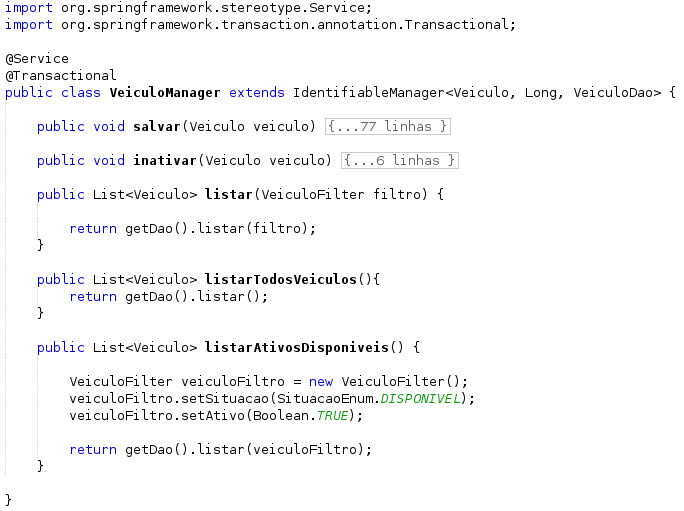
\includegraphics[width=0.75\textwidth]{dados/figuras/manager.png}
    \fonte{SEDES}
    \label{fig:figura-manager}
\end{figure}

\begin{figure}[!htb]
    \centering
    \caption{DAO Java - Veículo}
    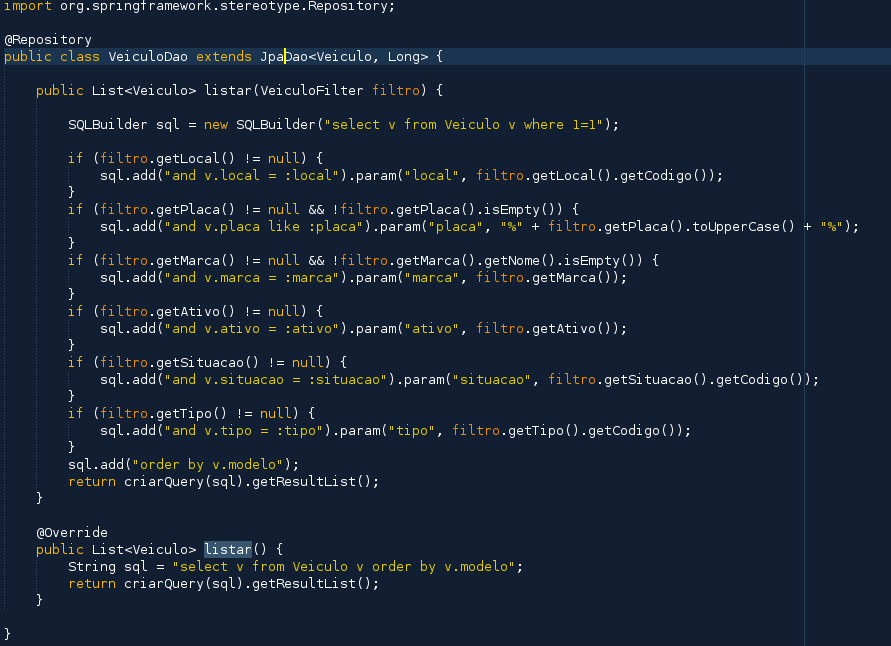
\includegraphics[width=0.75\textwidth]{dados/figuras/dao.png}
    \fonte{SEDES}
    \label{fig:figura-dao}
\end{figure}


\section{Homologação}
\label{sec:atividadesRealizadasHomologacao}

Ao final de cada Sprint é apresentada para o cliente uma prévia do que está sendo desenvolvido. A aplicação é então colocada em um servidor específico para sistemas em homologação rodando um Tomcat. Um schema no banco de dados também é criado e o código é compilado com as particularidades do ambiente de homologação que contém caminhos e usuários diferentes na rede para o banco de dados e servidores LDAP de autenticação. 

O desenvolvedor responsável pela homologação, em seu próprio computador muda, na IDE, o perfil de desenvolvimento para homologação e realiza o comando de compilação do código. Como resultado ele tem um arquivo no formato WAR e está pronto para realizar o "deploy" enviando o arquivo para servidor.

Em alguns casos a funcionalidade apresentada já pode ser utilizada para realizar cadastros pelo cliente e caso não aconteçam mudanças significativas no modelo esses dados podem ser importados quando a aplicação entrar em produção. 



\section{Documentação}
\label{sec:atividadesRealizadasDocumentacao}

A documentação ocorre após a apresentação das releases e aplicação dos ajustes, caso ocorram. O objetivo dessa tarefa é fazer a inclusão ou atualização do produto no catálogo de  produtos e a elaboração ou atualização do manual do usuário, que contempla as histórias implementadas e descreve passo a passo como realizar as tarefas. O manual é apresentado no formato PDF e é compilado junto com a aplicação que contém um link de ajuda apontando para o manual.


\section{Produção}
\label{sec:atividadesRealizadasProdução}

Após a entrega da última release prevista no escopo do projeto e a realização dos testes pelo cliente no servidor de homologação, já com as correções e ajustes sugeridas, ocorre a implantação da aplicação no servidor de produção. Um processo similar ao de implantação em homologação, porém com algumas particularidades.

Com o schema no banco de produção já criado e todas as tabelas e dados já implementados, o desenvolvedor responsável compila em sua IDE com o perfil de produção e realiza o deploy do aquivo WAR no servidor identificado pelo número da sua versão.

\begin{citacao}
... processo de levar código do desenvolvimento e teste para produção. É comum chamar esse processo de deploy em ambiente de
produção. Em português é até possível ouvir o neologismo deploiar, ou então o termo correto em português, que seria“implantar”. \cite[p.~19]{Sato2014}
\end{citacao}

A versão é numerada com dígitos na forma X.Y.Z. Os dois primeiros dígitos mais significativos (X e Y) são utilizados para incrementar o número de versão e o último (Z) para patches com correções de bugs. Uma  TAG\footnote{ É apenas um “snapshot” do projeto no tempo. http://svnbook.red-bean.com/en/1.7/svn.branchmerge.tags.html} é então criada no sistema de controle de versões SVN e contém o número de versão e sua descrição e serve para permitir recuperar o código-fonte, caso seja necessário, conforme a versão foi construída. O cliente é então informado formalmente que a versão está disponível para uso em produção.

\section{Encerramento}
\label{sec:atividadesRealizadasEncerramento}

A execução das atividades de finalização do projeto se iniciam com a formalização, pelo responsável de suporte de negócio, sobre discussões de melhorias do projeto, do modelo/arquitetura utilizada, dos  procedimentos, das técnicas e do método de desenvolvimento. 

O gerente do projeto realiza uma reunião final de entrega do produto com o time e o cliente, na qual deverá ser definido o responsável pelo suporte de negócio do produto. Preferencialmente, o gestor do sistema, ou alguém por ele delegado, deve assumir este papel, que consiste em esclarecer as dúvidas negociais reportadas pelos usuários do produto. À SEDES caberá o suporte técnico para correções e melhorias no sistema. Após a reunião comunica-se o encerramento do projeto aos interessados através de e-mail ou despacho/documento em processo administrativo.

As lições aprendidas deverão gerar oportunidades de melhorias que deverão ser incluídas no backlog de demandas da SEDES para implementação em momento oportuno e adoção em futuros projetos.